\documentclass[tikz,border=5mm]{standalone}
\usepackage{tikz}
\usetikzlibrary{positioning}

\begin{document}
\thispagestyle{empty}
    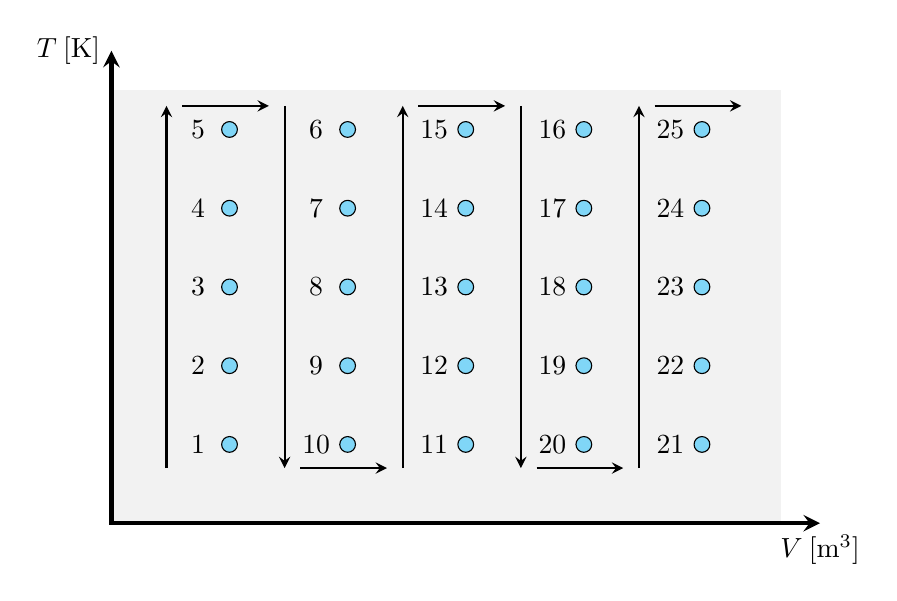
\begin{tikzpicture}
        \path [fill=white!90!gray] (0,0) rectangle (8.5,5.5);
        \draw [<->,>=stealth, ultra thick] (9,0) node[below]{$V \: \mathrm{[m^3]}$} -- (0,0) -- (0,6) node[left]{$T \: \mathrm{[K]}$};
        \draw [fill=white!50!cyan] (1.5,1) circle [radius=0.1] node at (1.1,1) {1};
        \draw [fill=white!50!cyan] (1.5,2) circle [radius=0.1] node at (1.1,2) {2};
        \draw [fill=white!50!cyan] (1.5,3) circle [radius=0.1] node at (1.1,3) {3};
        \draw [fill=white!50!cyan] (1.5,4) circle [radius=0.1] node at (1.1,4) {4};
        \draw [fill=white!50!cyan] (1.5,5) circle [radius=0.1] node at (1.1,5) {5};
        \draw [->,>=stealth, thick] (0.7,0.7) -- (0.7,5.3);
        \draw [->,>=stealth, thick] (0.9,5.3) -- (2.0,5.3);
        \draw [fill=white!50!cyan] (3.0,5) circle [radius=0.1] node at (2.6,5) {6};
        \draw [fill=white!50!cyan] (3.0,4) circle [radius=0.1] node at (2.6,4) {7};
        \draw [fill=white!50!cyan] (3.0,3) circle [radius=0.1] node at (2.6,3) {8};
        \draw [fill=white!50!cyan] (3.0,2) circle [radius=0.1] node at (2.6,2) {9};
        \draw [fill=white!50!cyan] (3.0,1) circle [radius=0.1] node at (2.6,1) {10};
        \draw [->,>=stealth, thick] (2.2,5.3) -- (2.2,0.7);
        \draw [->,>=stealth, thick] (2.4,0.7) -- (3.5,0.7);
        \draw [fill=white!50!cyan] (4.5,1) circle [radius=0.1] node at (4.1,1) {11};
        \draw [fill=white!50!cyan] (4.5,2) circle [radius=0.1] node at (4.1,2) {12};
        \draw [fill=white!50!cyan] (4.5,3) circle [radius=0.1] node at (4.1,3) {13};
        \draw [fill=white!50!cyan] (4.5,4) circle [radius=0.1] node at (4.1,4) {14};
        \draw [fill=white!50!cyan] (4.5,5) circle [radius=0.1] node at (4.1,5) {15};
        \draw [->,>=stealth, thick] (3.7,0.7) -- (3.7,5.3);
        \draw [->,>=stealth, thick] (3.9,5.3) -- (5.0,5.3);
        \draw [fill=white!50!cyan] (6.0,5) circle [radius=0.1] node at (5.6,5) {16};
        \draw [fill=white!50!cyan] (6.0,4) circle [radius=0.1] node at (5.6,4) {17};
        \draw [fill=white!50!cyan] (6.0,3) circle [radius=0.1] node at (5.6,3) {18};
        \draw [fill=white!50!cyan] (6.0,2) circle [radius=0.1] node at (5.6,2) {19};
        \draw [fill=white!50!cyan] (6.0,1) circle [radius=0.1] node at (5.6,1) {20};
        \draw [->,>=stealth, thick] (5.2,5.3) -- (5.2,0.7);
        \draw [->,>=stealth, thick] (5.4,0.7) -- (6.5,0.7);
        \draw [fill=white!50!cyan] (7.5,1) circle [radius=0.1] node at (7.1,1) {21};
        \draw [fill=white!50!cyan] (7.5,2) circle [radius=0.1] node at (7.1,2) {22};
        \draw [fill=white!50!cyan] (7.5,3) circle [radius=0.1] node at (7.1,3) {23};
        \draw [fill=white!50!cyan] (7.5,4) circle [radius=0.1] node at (7.1,4) {24};
        \draw [fill=white!50!cyan] (7.5,5) circle [radius=0.1] node at (7.1,5) {25};
        \draw [->,>=stealth, thick] (6.7,0.7) -- (6.7,5.3);
        \draw [->,>=stealth, thick] (6.9,5.3) -- (8.0,5.3);
    \end{tikzpicture}
\end{document}